\documentclass[12pt,a4paper]{report}

\usepackage{dolgozat}
\usepackage[]{algorithm2e}
\usepackage[breaklinks]{hyperref}
\usepackage{indentfirst}
\hypersetup{breaklinks=true}

\linespread{1.2}

\begin{document}

\include{cimlap/cimlap}

%Feladatkiiras
\begin{flushleft}
\textsc{\bfseries Miskolci Egyetem}\\
Gépészmérnöki és Informatikai Kar\\
Alkalmazott Matematikai Intézeti Tanszék\hspace*{4cm}\hfil \textbf{Szám:}
\end{flushleft}
\vskip 0.5cm
\begin{center}
\large\textsc{\bfseries Szakdolgozat Feladat}
\end{center}
\vskip 0.5cm
Árva Zoltán (B5X5NT) mérnökinformatikus jelölt részére.\newline

\noindent\textbf{A szakdolgozat tárgyköre:} Számítógépi grafika, optimalizálás, C++ programozás\newline

\noindent\textbf{A szakdolgozat címe:} Számítási modellek bemutatása egy FPS játék készítése kapcsán\newline

\noindent\textbf{A feladat részletezése:}

\bigskip

A számítógépes játékok különféle komplex számítási és programozási problémákat vetnek fel. Ilyenekkel a mérnöki gyakorlatban is napi szinten találkozhatunk.

\medskip

A dolgozat célja, hogy egy belső nézetes, lövöldözős játék elkészítése kapcsán bemutasson ezek közül néhányat, amelyek lehetnek például az alábbiak.

\begin{itemize}
\item Ütközésvizsgálat térben. Hatékonyság javítása térpartícionálási módszerekkel.
\item Útvonalkeresési módszerek egzakt és heurisztikus algoritmusokkal.
\item Interpolációs módszerek alkalmazása számítógépes játékok karaktereinek animálásához.
\item Döntési módszerek vizsgálata, alkalmazása a nem játékos karakterek viselkedésének modellezéséhez.
\end{itemize}

\vfill

\noindent\textbf{Témavezetõ:} Piller Imre (egyetemi tanársegéd) \newline

% \noindent\textbf{Konzulens(ek):} (akkor kötelezõ, ha a témavezetõ nem valamelyik matematikai tanszékrõl való; de persze lehet egyébként is)\newline

\noindent\textbf{A feladat kiadásának ideje:}\newline

%\noindent\textbf{A feladat beadásának határideje:}

\vskip 2cm

\hbox to \hsize{\hfil{\hbox to 6cm {\dotfill}\hbox to 1cm{}}}

\hbox to \hsize{\hfil\hbox to 3cm {szakfelelõs}\hbox to 2cm{}}

\newpage

\vspace*{1cm}  
\begin{center}
\large\textsc{\bfseries Eredetiségi Nyilatkozat}
\end{center}
\vspace*{2cm}  

Alulírott Árva Zoltán; Neptun-kód: B5X5NT, a Miskolci Egyetem Gépészmérnöki és Informatikai Karának végzõs mérnök informatikus szakos hallgatója ezennel büntetõjogi és fegyelmi felelõsségem tudatában nyilatkozom és aláírásommal igazolom, hogy "Számítási modellek bemutatása egy FPS játék készítése kapcsán" címû szakdolgozatom/diplomatervem saját, önálló munkám; az abban hivatkozott szakirodalom
felhasználása a forráskezelés szabályai szerint történt.\\

Tudomásul veszem, hogy szakdolgozat esetén plágiumnak számít:
\begin{itemize}
\item szószerinti idézet közlése idézõjel és hivatkozás megjelölése nélkül;
\item tartalmi idézet hivatkozás megjelölése nélkül;
\item más publikált gondolatainak saját gondolatként való feltüntetése.
\end{itemize}

Alulírott kijelentem, hogy a plágium fogalmát megismertem, és tudomásul veszem, hogy
plágium esetén szakdolgozatom visszautasításra kerül.

\vspace*{3cm}

\noindent Miskolc, 2017. év 11. hó 24. nap

\vspace*{3cm}

\hspace*{8cm}\begin{tabular}{c}
\hbox to 6cm{\dotfill}\\
Hallgató
\end{tabular}


\cleardoublepage
\pagenumbering{gobble}
\tableofcontents
\cleardoublepage
\pagenumbering{arabic}

\newpage

\pagestyle{myheadings}
\pagestyle{fancy}

\clearpage
\setcounter{page}{1}

\Chapter{Bevezetés}
\label{Chap:bevezetes}

% TODO: Bővíteni kellene még a végén szereplő kommentek szerint például.

Egy FPS (\textit{First-Person Shooter}) játék elkészítése különféle számítási- és optimalizálási problémákat vet fel. A számítógépes grafika és a játékfejlesztés segítségével lehetőség adódott a termelésinformatikához kapcsolódó optimalizálási problémák bemutatására.

Azon számítógépes játékoknak, amelyek célja a minél valószerűbb megjelenítés, számos olyan eleme van, amely optimalizálás nélkül olyan erőforrásigényes lenne, amely a manapság elérhető csúcskategóriás számítógépeken sem futna megfelelően. Ilyen elem például a karakterek mozgásterének definiálása, a lövés során eltalált objektumok metszéspontjának számítása, az ellenfelek viselkedésének szimulálása.

Megjelenítés szempontjából nagyon fontos, hogy a videokártyának megfelelő formátumban, egyben adjuk át a kirajzolni kívánt elemeket, mert így hatékonyabb lesz a megjelenítés, jobban ki lehet használni a rendelkezésre álló erőforrásokat, illetve a magasabb másodpercenkénti képkockaszámot.

A problémakör egyik fontos eleme az ellenfelek bejárható területének kezelése. Tulajdonképpen ez is egyfajta ütközésvizsgálatot jelent a falakra, objektumokra nézve. A dolgozatban bemutatásra kerülnek azon térpartícionálásos megoldások, amelyekkel a számítások gyorsabban, hatékonyabban elvégezhetők.

Az ütközésvizsgálat egy másik tipikus esete az ilyen jellegű játékokban a lövedékek útjának és metszéspontjainak kiszámítása. Ennél például jelentős optimalizációt érhetünk el, ha csak azon objektumokat vesszük figyelembe, amelyek a lövedék haladási irányába esnek.

% TODO: Hitbox-okról néhány dolog.

% TODO: Viselkedésmodellezésről kb. egy bekezdés még.

\Chapter{Problémakör}
\label{Chap:problemakor}

\section{Játékmotorok}

Új játék fejlesztésénél két fő lehetőség adott. Az első, hogy választunk egy kész, elérhető grafikus vagy játékmotort, amely majd a játék alapját adja. Amennyiben nem találunk megfelelőt, akkor írhatunk egyet saját magunknak.

% TODO: Kellene még hivatkozás az összes említett játékmotorra!

Meglévő motorok például az Unreal engine, Cryengine, Quake engine (ID Tech). Az Unreal engine első változata 1998-ban jelent meg, az első játék, amelyik ezt használta az Unreal nevű játék volt. A motor jelenlegi, legújabb verziója a 4.17-es. Nagyon sokat fejlődött az évek során.

% TODO: Az Unreal fejlődésével kapcsolatban lehet még említeni pár dolgot.

A Cryengine-t először a Far Cry (\ref{fig:farcry}. ábra) nevű játéknál használták 2004-ben, a második, illetve harmadik verziót pedig a Crysis trilógiához. Ezen játékok mindegyike a magas, korát megelőző grafikai megjelenésről lett híres, nagyon szép összképet lehet elérni ezzel a motorral.

% TODO: Itt is lehet még konkretizálni, hogy a szépsége miből adódik.

Az általam írt motorhoz a legközelebb a Quake engine (ID tech) 2-es és 3-mas verziója áll. Ezen motorok, összességében bármelyik megoldást is választjuk, a játékunk fő komponenseinek a háttérszámításait végzik, például lövés pályájának számítása, játék fizikájának számításai, ütközésdetektálás, billentyűzet és egérkezelés, hangokkal kapcsolatos számítások, hálózati kommunikáció, animációk, mesterséges intelligencia. A játékmotor kiválasztása vagy megírása után, a következő lépés a játék felépítése a motor adta eszközökkel. Praktikusan arra kell törekednünk, hogy olyan játékmotort válasszunk, amelyikben minél több kész funkció elérhető számunkra.

\begin{figure}[h]
\centering
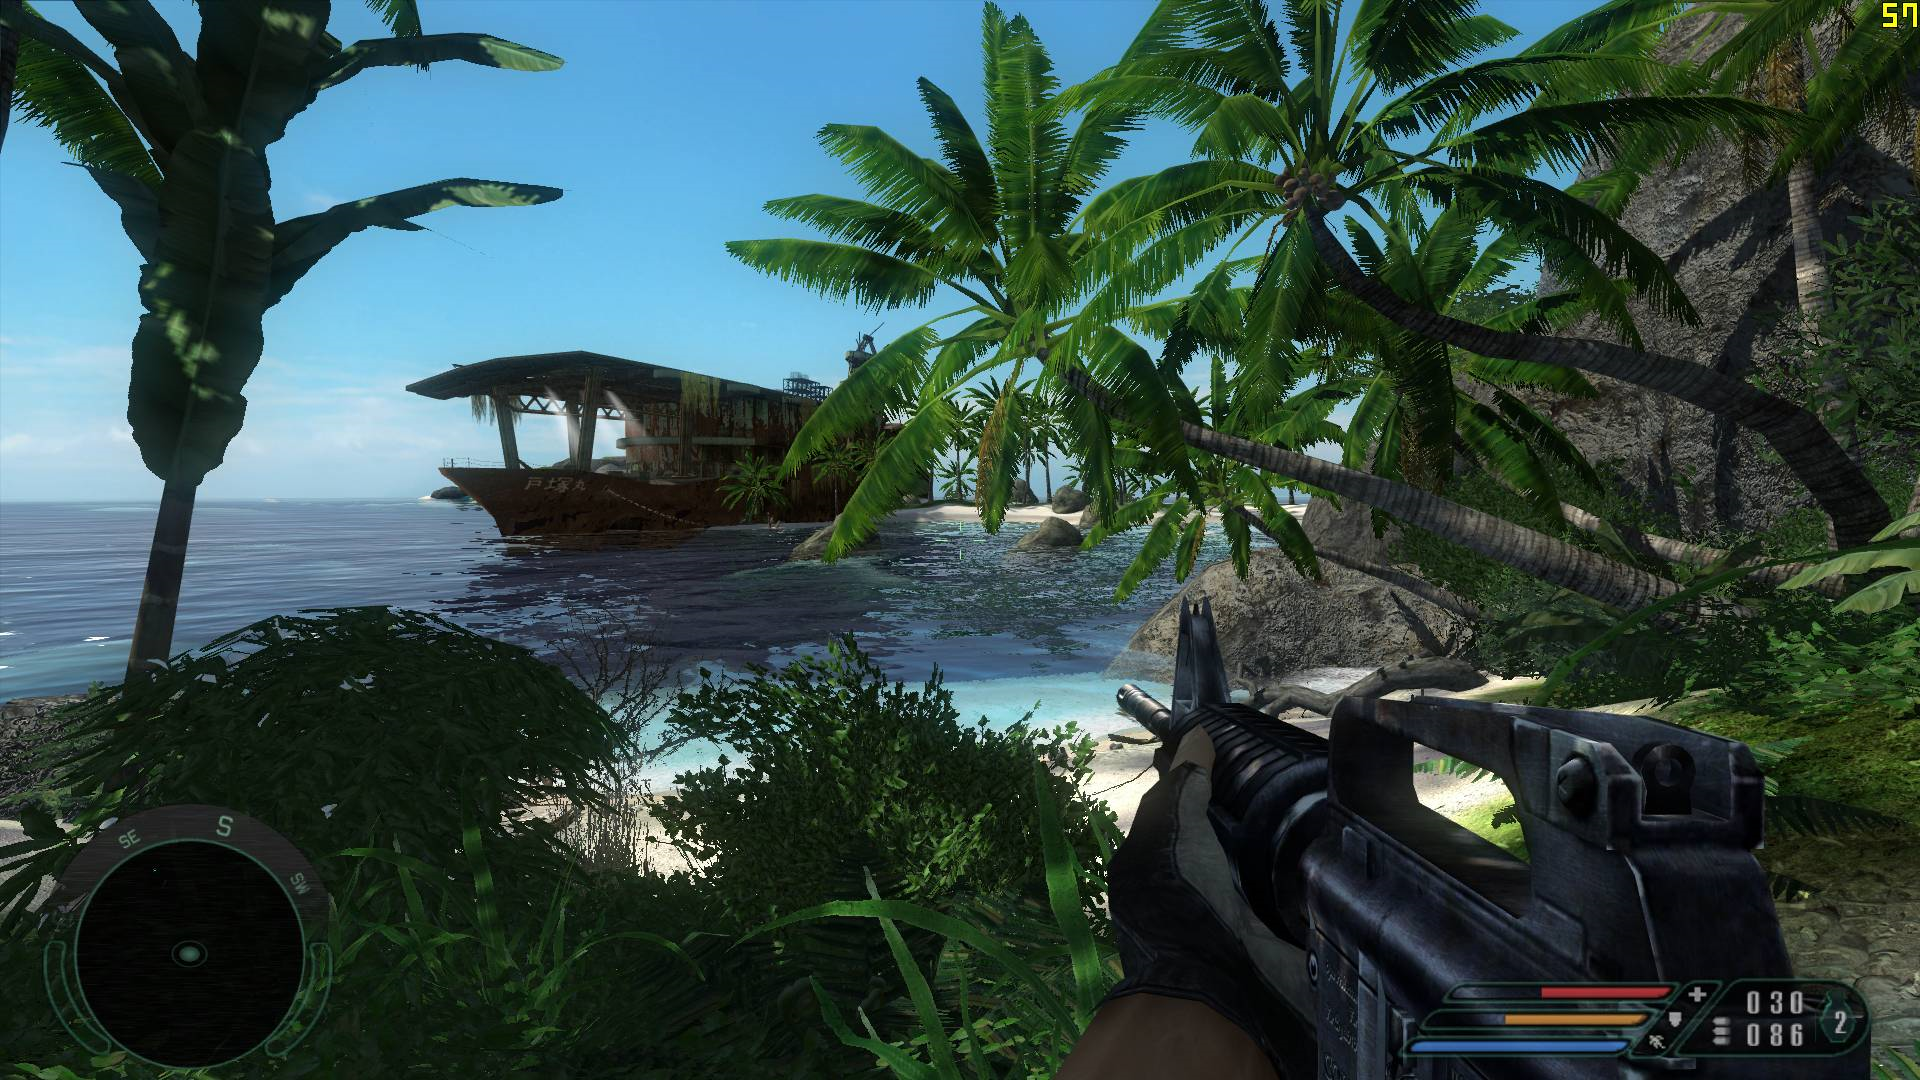
\includegraphics[scale=0.27]{kepek/farcry.png}
\caption{Pillanatkép a Far Cry című játékból (Crytek)}
\label{fig:farcry}
\end{figure}

\section{Egyedi igények és megoldandó problémák}

A saját játékom tervezésekor, megvizsgáltam, hogy milyen jellegű programra, milyen funkciókra van szükség, azt hogyan tervezem majd megvalósítani. Egy kész játékmotor használata helyett egy saját játékmotor implementálására esett a választás. A döntést részben az indokolta, hogy az egyedi funkciók implementálására egy kész játékmotor esetében is szükség lenne. A fő ok viszont az volt, hogy egy játékmotor fejlesztése kimondottan alkalmas különféle matematikával (geometriával, optimalizálással) és programfejlesztéssel (szoftver architektúrával és implementációval)  kapcsolatos problémák vizsgálatára, szemléltetésére és megoldására.

\section{Optimalizálási problémák}

A játékban megvalósítandó elemek között szerepel a lövés, a mesterséges intelligencia, az ütközésvizsgálat, és mindnek megvannak a maga optimalizálási problémái. Ütközésvizsgálatra szükség van a játékos karakterének az ellenfeleknek és a lövéshez is a találatok regisztrálására, pontos helyének számolására. A játéktér háromszögekből áll. A lövés megvalósításához szükségünk van háromszög, és egyenes metszéspontjának számítására, hogy vizualizálható legyen a lövedék becsapódásának helye a talajon, falakon, illetve egyéb játékbeli elemeken. Ez alapjában véve egy matematikai probléma, amit ki kell számoltatni, le kell programozni. Meg kell határozni azt az egyenest, ami azt mutatja meg, éppen merre nézünk, majd vizsgálni kell, hogy az adott egyenes metszi-e a teret alkotó háromszögek egyikét. De mivel több 100000 háromszög és egyenes metszéspontját kellene alap esetben számítani, így ez több optimalizálási problémát is felvet, amit a későbbiekben részletezek.

\section{A játékmotor fő elemei}

\subsection{Mesterséges intelligencia}

% TODO: Itt még nem ilyen, osztály szintjén kellene tárgyalni a dolgot. Az MI és az ütközésvizsgálat kapcsolatát kellene inkább részletezni kicsit.

Az MI osztálynak elsősorban az a feladata, hogy az ellenfelek egy meghatározott útvonalon mozogjanak, ne menjenek át falakon, menjenek egymásba. A véletlenszerűen lerakott ellenfelet a legközelebbi definiált waypoint-hoz kell irányítani, definiálni kell a célpontot (ami elsődlegesen a játékos), és ki kell számítani a pontokon keresztül vezető legrövidebb útvonalat.

\subsection{Hangok}

% TODO: A játékmotorok felsorolása után kellene egy részletesebb leírást csinálni az SDL-ről.

Egy játékhoz hozzátartoznak a hangeffektek, zenék is, amik élvezetessé teszik azt. Egy jól megválasztott zene például nagyon sokat tud javítani a játékélményen. Ezek megszólalásáért az SDL\_mixer felelős, ami lehetővé teszi azt is, hogy több hang egyidőben, átfedésben megszólaljon, és ne várják meg egymást. Ezt a Sound osztályban valósítottam meg. Lehetőség van hangcsatornákat megadni, folyamatos újrajátszást, illetve a hangok egymáshoz viszonyított hangerejét beállítani.

\subsection{Magasságmező}

% TODO: Itt sem kellene még belemenni az implementációba. Ami itt van, az elég, ha egy kicsit később szerepel majd. Ide az kellene, hogy a domborzat az mennyiben illeszkedik az eltervezett játék térképének kialakításához.

A játékteret adó domborzatot, a játék egy fekete-fehér, 384x384 pixeles képből számolja ki. Az adott képen minél magasabb egy pont, annál fehérebb, így a fehér adja a legmagasabb, a fekete szín a legalacsonyabb pontot. Ezekből az adatokból vissza lehet számolni a játékos függőleges pozícióját is, illetve az átmeneteket nézve, meredekségnek megfelelően a visszacsúszást. Mindez tehát megadja a játékteret minden szempontból (vizualitás, játékos mozgástere).

\subsection{Modellek kezelése}

% TODO: A modell tárolási formátumot kellene kicsit pontosítani!

A játéktér adatait tehát képből kinyertük, de ez még nem jelenti azt, hogy látjuk is a monitoron. Ehhez a VBO-s (Vertex Buffer Object) kirajzolási módszert választottam, ami a videókártyának a legoptimálisabb adatstruktúrában adja át azt a lehető leggyorsabb kirajzoláshoz.

\subsection{A csapda, mint játékelem}

Mindenképp szerettem volna olyan elemet a játékba, ami megkülönbözteti a többi, hasonló, aréna jellegű, túlélős játéktól. Az egyik ilyen elem, hogy ha a játékos egy előre meghatározott időnél több ideig nem mozdul, akkor megjelenik alatta egy csapda, amelybe leesik, és meghal. Vannak olyan játékok, ahol szimplán az ellenfelek ösztönzik a játékost a mozgásra, de a játék itt kikényszeríti azt, hogy a játékosok mozgásban legyenek. A megállásnál a küszöbérték tapasztalati alapon beállítva 5 másodperc lett. Ezt követően megjelenik a csapda modell egy hang kíséretében. Ezt követően 2 másodpercig még a kamera irányát tudja változtatni a játékos, utána viszont már azt sem. Ezt követően az a föld felé fordul, majd értesíti a játékost a történtek okáról.

\subsection{A lövés}

Egy ilyen játékban alapelem az is, hogy tudjunk lőni, mivel e nélkül az egész értelmét vesztené. A játéktér alapvetően egy textúrázott polygonháló. A lövés során azt kell meghatározni, hogy a lövedék melyik háromszögbe ütközne bele, ha a nézet irányába lőnénk, és egyenes pályát feltételeznénk. Ez egy olyan metszéspontszámítást tesz szükségessé, amelyet a játék összes objektumára el kell végeznünk. Megjelenítés szempontjából ez tipikusan egy lövés textúra illesztését jelenti.

% TODO: Az ellenfelekre vonatkozó ütközésvizsgálatnál a hitbox csak addig kell, amíg azt meg sikerül állapítani, hogy a tartalmazó hitbox-ot eltalálta-e a lövés. Azt követően már a konkrét modellre is meg lehet csinálni a vizsgálatot.

\section{A játék szabályai és mechanikája}

Egy belső nézetes lövöldözős játék esetében az adott személy szemszögéből látjuk a virtuális világot. Egy olyan, aréna jellegű, túlélő játékról van szó, amelyben a játékosok mesterséges intelligenciával rendelkező ellenfelekkel (gyakori szóhasználat szerint \textit{bot}-okkal) harcolnak.

A játék során az ellenfelek hullámokban érkeznek. Egy ilyen hullám akkor ér véget, ha a játékosnak megadott számú ellenfelet sikerült eltalálnia. Közben a játékosnak lehetősége van gyógyszert és lőszert szereznie. A játékos teljesítményének függvényében a fegyver fejlesztését is lehetővé teszi a játék.

A klasszikusan felszedhető tárgyak (\textit{powerup}-ok) mellett a játékban, az előzőekhez kinézetükben hasonló csapda jellegű elemek is vannak. A felszedhető elemek hatása így tehát lehet egyaránt pozitív vagy negatív.

A játék megvalósításának problémaköre tehát szerteágazó. Többek között meg kellett valósítani a modellbetöltést textúrázással, az irányítást, fizikát, ütközéskezelést, ellenfelek viselkedésének modellezését, fények és hangok kezelését.


\Chapter{Komponensek}
\label{Chap:komponensek}

- Felhasznált technológiák (C++, SDL)
- Nagyobb komponensek

Le kellene írni, hogy hogyan épül fel a program. Milyen nagyobb modulokból épül fel.

A játék indításának a folyamatát is lehetne részletezni.

\Chapter{Ütközésvizsgálat}
\label{Chap:utkozesvizsgalat}

% TODO: Ütközéssel, metszéspontokkal kapcsolatos számítások

%- A try bullet-es példa részletes kifejtése, matematikai része

%Egyszerűbb változatoktól a bonyolultabbak fel

%- Először az intuitív, egyszerűbb megoldások, még ha kevésbé hatékony is.
%- Felsorolni több megoldást is.
%- Optimalizálási módszerek részletezése
%- Összehasonlítani őket pontosság és számításigény szempontjából.

Ebben a fejezetben az ütközésvizsgálattal kapcsolatos számításokról, optimalizációkról lesz szó. Ütközésvizsgálatra több szempontból is szükség van. Egyrészt, vizsgálni kell, hogy a játékos a játszható területen belül van-e, azaz nem mehet át falakon, tereptárgyakon, nem mehet fel túl meredek emelkedőn. Másrészt, vizsgálni kell, hogy a játékos által leadott lövedék eltalálja-e a domborzatot, tereptárgyakat, jelezni kell a lövedék becsapódását. Harmadrészt regisztrálni kell az ellenfeleket eltaláló leadott lövéseket. A második és harmadik pont nagyon hasonló, de még is szétszedtem, mert az ellenfeleknél nem a látható geometriát találjuk el, hanem annak egy leegyszerűsített modelljét, a számítások felgyorsítása érdekében. Szükség van további optimalizációkra is, mert ha ezek nem lennének, irreálisan nagy erőforrás igénye lenne a játékoknak.

\section{A karakterek ütközésvizsgálata mozgás szempontjából}

Ez a játék szempontjából az egyik legfontosabb elem. Az hogy kirajzoltatunk valamit a képernyőre, még nem jelenti azt, hogy azon nem lehet áthaladni. A kirajzolás csak a vizualitást adja, a domborzat, a tereptárgyak, a karakterek kinézetét. A játékfejlesztő feladata az, hogy megírja külön az ezekhez szükséges ütközésvizsgálatot. Mivel ez két különálló dolog, egyes helyzetekben adódhatnak olyan problémák, hogy ezek nincsenek szinkronban, tehát látunk valamit amin át lehet menni, vagy nem látunk valamit és mégis megakadunk benne.

Ebben a játékban a karakterek ütközésvizsgálata gradiens számítással van megoldva. Ez azt jelenti, hogy ha két, egymás mellett lévő pont magasságértéke között túl nagy a különbség pozitív irányba, az falat, vagy túl meredek emelkedőt jelent. Ha mérsékelt, vagy nagyon minimális a különbség, akkor arról vagy lecsúszik, vagy csak egyszerűen át lehet ott haladni. Mindezt a beolvasott magasságmezőből számolja, ezzel dinamikussá téve az ütközésvizsgálatot. Ha ez nem lenne így, akkor elveszne a játék azon tulajdonsága, hogy dinamikusan lehet cserélgetni a pályákat minden további nélkül.

Ezen felül a gravitáció ami nagyon lényeges, mert a pályának vannak olyan magaslati pontjai, amelyekre fel lehet jutni. Ha egy ilyenre felmegyünk, és nincs semmilyen erő, ami a karaktert a föld felé húzná, akkor felfelé ugyan lekövetné a talajmagasságot, de le már nem esne alacsonyabb pontra onnan.

 Ez esetben egy lefelé ható erő folyamatosan hat a játékosra és ellenfelekre, aminek a küszöbértéke mindig az aktuális talajmagasság. Ennek pszeudokódja:

\begin{verbatim}
1. gravitációs erő := -9,8;
2. küszöbérték := aktuális talajmagasság;
3. ha karakter függőleges pozíciója > küszöbérték
4. 	akkor
5.		függőleges gyorsaság = függőleges gyorsaság + gravitációs erő;
6.		karakter függőleges pozíciója = karakter függőleges pozíciója 
										+ függőleges gyorsaság;
6.	különben
7. 		karakter függőleges pozíciója = küszöbérték;
\end{verbatim}
 
\section{A domborzat és tereptárgyak üközésvizsgálata a lövés szempontjából}

Az ilyen fajta ütközésvizsgálat számítás nem létszükséglet a játszhatóság szempontjából, de tény, hogy jóval realisztikusabbá teszi a játékot, és sok optimalizációt igényel. Ez teszi lehetővé, hogy ha lövünk egyet, és beletalál bármilyen elembe, ami a pálya része, megjeleníthessük rajta a találatot. Ennek minősége lehet többféle, csak egy textúra, vagy egyéb még realisztikusabb megoldások.

\begin{figure}[h]
\centering
\includegraphics[scale=0.4]{kepek/map_wireframe.png}
\caption{A térkép geometriájának határvonalai}
\label{fig:wireframe}
\end{figure}



\section{A játékos, és az ellenfelek hitboxa}

f



\Chapter{Útvonalkeresés}
\label{Chap:utvonalkereses}

A fejezet az útvonalkeresésnél alkalmazott módszereket mutatja be.

\section{A waypoint-ok fogalma és jellemzői}

Ez egy térben meghatározott egyszerű pont, amely nem látható a játékos számára. A mesterséges intelligencia ezeket használja fel az ellenfelek mozgatásához. Azért van rájuk szükség, mert a pályán vannak falak, különböző játékelemek, amiken nem lehet átmenni, és ezekkel a pontokkal egyértelműen meg lehet határozni, hogy melyek azok a helyek, amelyek bejárhatók.

A waypoint-okhoz rendelhetünk különféle többletinformációkat. Ilyenek lehet például, hogy az adott pontban a gépi játékosnak megállnia, guggolnia.

\section{A waypoint-hoz tartozó adatok}

A waypoint-ok pozícióját két dimenziós Descartes koordináta rendszerben $(x, y)$ koordinátákkal adhatjuk meg. Annak ellenére, hogy térben vagyunk, nincs szükség $z$ koordinátára, mert a talaj magassága külön kezelendő, mivel az hatással lesz az ellenfelek viselkedésére. Ennek köszönhetően mindig az adott pálya talajmagasságához tud igazodni, nem szükséges azt külön megadni.

Fontos, hogy a waypoint-nak legyen egy típusa, amely meghatározza, hogy az adott pont milyen szerepet játszik. Ennek segítségével ki lehet számolni, hogy a játékban szereplő karakterek hova mehetnek.

\section{Útvonalkeresés waypoint-ok alapján}

Tegyük fel, a gép létrehoz egy ellenfelet egy véletlenszerű pozícióba. (Ezt a szakzsargonban \textit{spawn}-olásnak hívják.) Az ellenfeleknek az a fő feladatuk, hogy a lehető legrövidebb útvonalon eljussanak a játékoshoz, és megtámadják. 

Az útvonalkeresés folyamata a következő fő lépésekből épül fel.
\begin{itemize}
\item A waypoint-ok közül megkeressük az adott karakterhez vagy objektumhoz legközelebbit. Először ezt a pontot kell megközelíteni.
\item A waypoint-ok közül meghatározzuk a célponthoz legközelebbit, ez lesz majd a célpont.
\item A pont adott, kis sugarú környezetét elérve A*-algoritmus segítségével meghatározzuk a legrövidebb útvonalat.
\item A célpontot elérve már csak az adott karakterhez vagy objektumhoz kell egyenes úton eljutni.
\end{itemize}

% TODO: Készíteni egy demo-t az A*-algoritmushoz, és megnézni, hogy a legközelebbi pontok keresése pontosan hogy nézne ki, és egyáltalán kell-e hozzá külön heurisztika.

\begin{algorithm}[H]
 \KwData{Waypoint vegso\_pont\;\\ Vec2 legkozelebbi\_pont\;\\double pont\_tav, temp, x\_tav, y\_tav\;\\ float x, y\; }
 \KwResult{Legközelebbi pont x és y koordinátája}
 pont\_tav := 100000\;
 \For {Waypoint pont : waypointokon}{
 	x := pont.x;\\
	y := pont.y;\\
	x\_tav := |(x – jelenlegi\_xpoz)|;\\
	y\_tav := |(y – jelenlegi\_ypoz)|;\\
	temp := sqrtf(x\_tav * x\_tav +  y\_tav * y\_tav)\;
  \If{temp < pont\_tav}{
   		pont\_tav := temp;\\
		vegso\_pont := pont\;
   }
   legkozelebbi\_pont.x := vegso\_pont.x;\\
   legkozelebbi\_pont.y := vegso\_pont.y\;
 }
 \caption{A legközelebbi pont megkeresése}
\end{algorithm} 

\section{Az A*-algoritmus}

% TODO: Keresni A*-algoritmusos irodalmat/hivatkozást.

Ezt az algoritmust a legrövidebb útvonal számításra gyakran használják, mert ez az egyik leghatékonyabb. Bemeneti paraméterei a start pont X, Y, és a célpont X, Y koordinátái. 

A keresést egy gráfon tudjuk végrehajtani. A gráf egy lehetséges realizációja a rács, amelyben a gráf pontjai négyzetrácsnak megfelelően helyezkednek el.

Ez a rácsos kialakítás több szempontból is előnyös. A pontok minden esetben egymástól egyforma távolságra helyezkednek el, így ezeket nem kell számolni. Továbbá ha csak a bejárható helyekre helyeznénk pontokat, külön olyan algoritmusra lenne szükség, amely meghatározza azt, hogy melyik pontból melyikbe haladhatunk. Pontpárok tárolására lenne szükség, amelynek a pálya elrendezéséhez való dinamikus meghatározása plusz erőforrásigény. A rácsos megoldással a pálya elrendezésétől függetlenül rakjuk le a pontokat, csak egy értéket állítunk át a pont típusának megváltoztatásakor, amely a be nem járható területeket határozza meg.

Listát kell vezetni azon pontokról amiket még nem jártunk be, illetve azokról is, amelyeket bejártunk, ezeket hívjuk nyitott (Open) illetve zárt(Closed) node listáknak. A nyitott node lista másképpen fogalmazva a hátralévő, vizsgálatlan pontok, a zárt node lista pedig a már vizsgált pontok halmaza. Kell lennie egy, vagy több feltételnek, hogy az adott pontból merre haladhatunk tovább, ilyen például az, hogy csak vízszintesen és függőlegesen haladhatunk a ponthálón, vagy átlósan is.  Az a pont, amin éppen tartózkodunk az a jelenlegi node (current node), amelyekre léphetünk, azok pedig a gyerek node-ok (successor node).

Egy node-hoz a következők tartoznak: X és Y pozíció, ezen felül kell lennie egy változónak, amiben az adott pontig bejárt távolság található. Illetve le kell tárolni egy prioritás változót is, amiben az eddig megtett út, és a még hátralevő út távolságainak összege található.
Fontos ugyanis az algoritmus működése szempontjából az eddig megtett, és a hátralévő út, ugyanis ezekből az adatokból számolja ki egy adott pont prioritását (kezdőponttól való táv + célponttól való táv), és így dönti el milyen pontokat részesítsen előnyben. A prioritás minél kisebb érték, annál jobb, szóval arra kell elindulni. Ha egy idő után falba ütközik, elkezdi vizsgálni mindig a lehető legkisebb prioritással rendelkező, még szabad pontokat, egészen addig, még utat nem talál valahol magának.

Az A* algoritmus leírása pszeudokóddal:
A célpontot jelöljük goal\_node-dal, a kezdőpontot pedig start\_node-dal.

\begin{verbatim} 
1.Helyezük a start_node-ot az Open listába. f(start_node)=h(start_node)
2.Amíg az Open lista nem üres
3.	Vegyük a az Open listából azt a node-ot, amely a legkisebb költségű
4.		f(current_node) = g(current_node) + h(current_node)
5.	ha current_node a célpont, megtaláltuk a megoldást; break
6.	Generáljunk minden állapothoz successor_node-ot, ami a 
		current_node-ból származik
7.	ciklus minden current_node successor_node-ján
8.		Állítsuk be a successor_current_költséget, amely g(current_node) 
				+ w(current_node, successor_node)
9.		ha successor_node az Open listában van
10.			ha g(successor_node) <= successor_current_költség ugrás 19-re
11.			különben ha successor_node a Closed listában van
12.			ha g(successor_node) <= successor_current_költség ugrás 19-re
13.			Mozgassuk successor_node-ot a Closed listából az Open listába
14.		    különben
15.			Adjuk hozzá successor_node-ot az Open listához
16.			Állítsuk a h(successor_node)-ot hogy megkapjuk a heurisztikus 
				távolságot a célig
17.		Legyen egyenlő g(successor_node) a successor_current_költséggel
18.		Állítsuk be node_successor szülőjét current_node-nak
19.	Adjuk hozzá a current_node-ot a Closed listához
20.ha(current_node != goal_node) lépjünk ki a következővel: 
						(az Open lista üres)
\end{verbatim}

\section{A pontos megvalósítás}

A program a játéktér alapját képző domborzatot, egy képből olvassa be. Ez a magasságmező, ahol egy adott pont magasságát a világossága határozza meg, minél világosabb, annál magasabb pontot jelent a domborzaton, így 256 féle magasság lehetséges, ami az aktuális változathoz megfelelő felbontásnak bizonyult. 

A játéktér jelentős része (körülbelül 95\%) bejárható. A magasságmezőhöz tartozó kép felbontása $384 \times 384$ pixel, amely a térkép megfelelő részletességű megjelenítése miatt ennyi. A waypoint-ok meghatározására több lehetőség is van.

Az egyik lehetőség, ha minden pixelhez rendelünk egy pontot. Ez olyan szempontból lehet előny, hogy pontosabban meg van határozva az összes pont amelyre léphet az ellenfél. Hátránya viszont, hogy ez nagyon sok számításigény, és fölösleges is minden pixelre egy waypoint.

A másik lehetőség, ha 8 pixelenként határozunk meg egy waypoint-ot, ami 48x48-as felbontást eredményez. Azért pont erre az értékre esett a választásom, mert ez nagyban gyorsítja a számításokat, viszont még nem megy a bejárható területek rovására, megfelelően pontos. Ez kevesebb memória igényt jelent, és mivel kevesebb adattal is kell számolni, kevésbé terheli a processzort is. Ez látható \aref{fig:diagram_utvonal} ábrán.

\begin{figure}[h]
\centering
\includegraphics[scale=0.9]{kepek/utvonal_szamitas_diagram_waypointokra.png}
\caption{Számításigény a felbontás és idő függvényében}
\label{fig:diagram_utvonal}
\end{figure}

Első lépésként, létre kell hozni a waypoint hálót, amiken a mesterséges intelligencia végig fog menni, elkerülvén hogy átmenjen a tereptárgyakon, falakon. Ezek a pontok 8 pixelenként, függetlenül az adott pixel színétől meghatározásra kerülnek, viszont a típusa az adott pixel színének megfelelően lesz beállítva. Ahogy \aref{fig:kuszobertek}-as ábrán is látható, a például egy pont színéből 50-nél nagyobb érték jön ki, akkor a pont típusa zártra állítódik, így ebbe az irányba nem lesz lehetséges a továbbhaladás. \aref{fig:mi_printscreen}  képen „.”-al a bejárható terület, „X”-el a falak, „S”-el az indulópont, „F”-el a célpont, „R”-el a legrövidebb útvonal van jelölve.

\begin{figure}[h]
\centering
\includegraphics[scale=0.22]{kepek/mi_printscreen.png}
\caption{Útvonal meghatározó algoritmus működése}
\label{fig:mi_printscreen}
\end{figure}

A képen még csak statikusan vannak megadva a falak, de mint ahogy fentebb olvasható, a játékon belül a beolvasott magasságmező színe határozza ezt meg. Erre azért van szükség, mert így lehet megoldani azt, hogy a mesterséges intelligencia alkalmazkodjon a környezetéhez. Ha a pályától függetlenül, statikusan lenne az összes waypoint típusa meghatározva, akkor ha a játékos más pályát rajzol, a pontok típusai nem illeszkednének az elrendezésre. Ezt a módszert alkalmazva, meg lehet adni, hogy egy bizonyos magasságnál csak másszon, vagy ugorjon, vagy bármilyen más tevékenységet végezzen. Ez egy fontos tulajdonsága a játéknak, mert azt úgy terveztem, hogy ha a felhasználó akár paint-ben rajzol egy pályát, akkor a teret azonnal kialakítsa, beállítsa hogy a falakon a játékos ne tudjon átmenni, a meredek lejtőkről visszacsússzon, illetve a mesterséges intelligencia is alkalmazkodjon.

\begin{figure}[h]
\centering
\includegraphics[scale=0.42]{kepek/magassagmezo_kuszobertek_diagram.png}
\caption{Küszöbérték a még bejárható terület meghatározásához}
\label{fig:kuszobertek}
\end{figure}

De a küszöbérték megadása nem mindig elegendő, ugyanis lehetnek olyan helyek a pályán, amelyek fal magasságúak, de bejárhatók, mert alacsony meredekségű emelkedő vezet fel oda. Ezt a problémát gradiens számítással lehet megoldani, ezzel van megoldva az is, hogy a játékos ne tudjon kimenni a játéktérből. Ahol túl nagy a meredekség, ott a waypoint típusát nem bejárhatóra kell állítani.

A pontok típusának a pálya alapján legenerálása után, az A*-algoritmus segítségével meghatározza a program a legrövidebb útvonalat a cél waypointig, természetesen a pontok típusait figyelembe véve. Ezt másodpercenként legalább 15x újra kell számolni, ugyanis a játékos mozog, és a cél waypoint mindig a játékoshoz legközelebb eső pont, ami ezzel együtt változik.

\Chapter{Animáció}
\label{Chap:animacio}

A fejezet a játékokban alkalmazott animációs módszereket, illetve azok megvalósítási módját mutatja be.

\Section{Kulcsképkocka alapú animáció}

Kulcsképkocka alapú mozgatást több területen használnak, például filmek készítésénél vagy játékok fejlesztésénél. Bármilyen célra is használjuk, az elv nem változik. Meg kell adnunk olyan pontokat, amelyeken szeretnénk ha az adott tárgy, vagy objektum áthaladna. Ezzel egy előre meghatározott mozgási útvonalat adunk meg. Az egyszerűbb animációknál egy alapállapot és egy végállapot van megadva, ilyen lehet egy redőny leengedése és felhúzása, ajtó vagy kapu kinyitása, becsukása. Ilyen jellegű, alap szintű animációknál, például ha egy redőnyt le akarunk engedni, annyi a dolgunk hogy megadjuk a kezdő és végpontot, majd idő paraméter szerint interpolálni. Ahogy az \aref{fig:keyframe} ábrán látható, ez a kulcsképkockák közötti mozgást eredményezi.

\begin{figure}[h]
\centering
\includegraphics[scale=0.5]{kepek/keyframe_anim.png}
\caption{Kulcsképkocka alapú animáció}
\label{fig:keyframe}
\end{figure}

A vertex alapú animációt a 3D játékfejlesztésben karakterek mozgatásához a 2000-es évek elejéig használták. Megvalósítása egyszerűbb, viszont sok memóriát igényel a tárolása, és nem eredményez olyan természetes mozgást általában, mint a csontváz alapú animáció. Ezt a technológiát többek között a Quake 1, 2 és 3 alkalmazta.

\SubSection{Az md2-es formátum}

Az md2-es modelltárolási formátumot az \textit{idSoftware} fejlesztette ki 1997-ben a Quake 2 nevű játékához. A formátum kulcsképkocka animációk tárolására alkalmas. Tartalmazza az adott modell geometriáit, és a képkockánkénti animációkat. 

A fájl adatai olyan struktúrában helyezkednek el, hogy könnyedén kirajzoltatható legyen a \texttt{GL\_TRIANGLE\_FAN} és \texttt{GL\_TRIANGLE\_STRIP} OpenGL függvényekkel. A formátum két fő részből áll: fejlécből és adatrészből. A fájl nem tartalmazza a modellek textúráját.

A fejléc egy struktúra, amely a fájl elején kezdődik, és tartalmazza az összes, feldolgozás szempontjából lényeges információt a fájl egészéről. Ilyen például a textúra szélessége, magassága, egy képkocka mérete, képkockák száma.

\Section{Csontváz alapú animáció}

A legtöbb mai játék ezt a módszert alkalmazza karakterek mozgatásához. Az alapötlete az, hogy a mozgatható részeket hierarchiába szervezi. Az élőlények felépítése általában olyan, hogy ezzel a fajta animálási móddal egyszerűen modellezhetők. 

A csontváz alapú animáció kapcsolódási pontokból (\textit{joint}-okból) építkezik. Ember esetén például a kézfej kapcsolatban van az alkarral, az alkar a felkarral, ami pedig a test többi részével. Minden hajlási pont egy új kapcsolódási pontot jelent. Tehát ha az ember felkarját megmozdítjuk, mozdul vele a kezének a többi része is. Ezt szemlélteti \aref{fig:skeletal}. ábra.

\begin{figure}[h]
\centering
\includegraphics[scale=0.5]{kepek/skeletal_anim.png}
\caption[]{Testrészek hierarchikus kapcsolódási pontjai emberen\footnotemark}
\label{fig:skeletal}
\end{figure}

\footnotetext{forrás: https://www.openflipper.org/media/plugin\_images/skeletalAnimation.png}

Szerencsére a módszer nem csak élőlények modellezésére alkalmazható hatékonyan. A naprendszerünk szintén modellezhető ilyen módon. Vannak a naprendszerünk bolygói, amelyek a tengelyük, és a központi csillag, a Nap körül is forognak.

Előnye, hogy könnyen létre lehet így hozni dinamikus animációkat, mivel az összes karakter csontjait lehet forgatni, mozgatni, továbbá megkönnyíti a bonyolultabb animációk elkészítését. Hátránya viszont, hogy komplexebbek, így több processzoridőt igényelnek.

\SubSection{Program: Emberszerű karakter animálása}

Az \texttt{Animáció} nevű programnak az a célja, hogy bemutasson egy animációs módszert, amelyet bárki fel tud használni karakteranimációhoz játékfejlesztésnél. Az animációt megvalósító algoritmus hasznos lehet még egy automatizált gyártósor robotkarjainak mozgatásához is olyan esetekben, amikor például két vagy több karnak mindig egy adott szög tartása mellett, összehangolva kell mozogniuk. A \texttt{Character} osztályban az összes mozgatással és azok pontos megjelenítésével kapcsolatos számítások találhatók. Az \texttt{Action} az állapotok kezeléséért, a \texttt{ModelLoader} és a \texttt{VboDrawer} a modellek (testrészek) betöltéséért, kirajzolásáért felelős, amelyeket a \texttt{MainGame} osztály fog össze. A konkrét felépítés \aref{fig:anim_uml} ábrán látható.

\begin{figure}[h]
\centering
\includegraphics[scale=0.6]{kepek/animation_uml.png}
\caption[]{Az animációt bemutató demó felépítése}
\label{fig:anim_uml}
\end{figure}

\Aref{fig:anim_demo} ábrán látható, futó programban egy egyszerű robotot tudunk irányítani, illetve ha a kamerát szabad mozgás módba váltjuk, meg tudjuk tekinteni a testrészek hierarchikus mozgását több szögből is. A robot részei több .obj kiterjesztésű modellből vannak betöltve, amelyek azért vannak külön modellben tárolva, hogy egymástól függetlenül tudjuk őket mozgatni, ne csak egyben a teljes robotot. A törzshöz csatlakozik a fej, a két kéz, és a két láb. Utóbbi kettő mindig 60 fokos szögkülönbséggel rendelkezik, és ha elérik a maximális, előre megadott kitérési értéket, a mozgás iránya megfordul. Az elérni kívánt mozgásmechanika implementálása után, meg kell adnunk a testrészek pozícióját. A \texttt{Character} oszályban lévő \textsl{BuildParts()} függvény a \texttt{ModelLoader} és a \texttt{VboDrawer} által betöltött és kirajzolt részek megfelelő pozícióba való elhelyezéséért felel, hogy azok egy egész robottá álljanak össze.

Járás közben az adott karakter előre is halad, illetve minimálisan fel és lefelé is mozog a járásból adódóan, és a testrészek fix szögben való mozgatásán kívül definiálnunk kell ezeket is. Figyelni kell, és számításba kell venni azt a jelenséget is, hogy járás közben egy élő ember  földre leért lába fix, azzal lendíti előre magát, így a láb végéhez képest kell megadnunk a hierarchiában feljebb lévő testrészek mozgását is, ezt nevezzük inverz kinematikának. Az előre és a fel-le irányba való mozgást a következő összefüggéssel írhatjuk fel:
$$
\Delta f = \left|
d \cdot \sin(\alpha)
\right|, \quad u = d \cdot \cos(\alpha),
$$

ahol $\Delta f$ az időegység alatt megtett előre mozgásnak a mértéke (\textit{forward}), az $u$ pedig a karakter fel-le mozgásának animálásához szükséges érték (\textit{up}). A $d$ az egységnyi idő alatt megtett távolságot jelöli (\textit{distance}), az $\alpha$ pedig a jobbláb animálásánál figyelembe vett szög értéke.

Az animálásért felelős részek időfüggőek, ugyanis garantálni kell hogy a különböző teljesítményű gépeken ugyanolyan gyors legyen az animáció. A két kirajzolt képkocka közötti eltelt időt a \texttt{CalcElapsedTime} függvény számolja, amelynek a kimeneti értéke az $s = v \cdot t$ képlettel számolható, ahol $s$ a megtett út, $v$ a sebesség, $t$ pedig az eltelt idő. Minél több a másodpercenként megjelenített képkockák száma, annál kisebb a köztük eltelt idő, és a mozgást annál kisebb értékkel szorozza be, így minden esetben ugyanolyan gyorsan fog mozogni az objektumunk, csak az animáció folytonosságában lesz különbség.

\begin{figure}[h]
\centering
\includegraphics[scale=0.4]{kepek/animation_demo.png}
\caption[]{Pillanatkép az animációt bemutató demóból}
\label{fig:anim_demo}
\end{figure}

A kamera alapesetben a robot mögött van, és annak mozgását követi, amelyet szintén a felhasználó tud irányítani. Az animáció bármikor félbeszakítható, nem áll vissza az alapértelmezett állásba, hogy megtekinthető legyen a mozgás minden fázisa.

\Section{Interpolációs módszerek}

Animációkészítés során többféle interpolációt használhatunk, ami azt jelenti, hogy ismert értékek alapján, a közbülső pontokra, vagyis nem ismert értékekre adunk közelítést \cite{curves}.

Különféle interpolációs módszerek vannak. A választás közülük nyilván attól függ, hogy pontosan mit szeretnénk megvalósítani. Egyszerűbb esetekben még megfelelő a lineáris interpoláció, viszont általában túlságosan szögletes mozgást eredményez, ezért valamilyen simább görbével való útvonal közelítést érdemes használni.

\SubSection{Lineáris interpoláció}

Ez a legegyszerűbb interpolációs módszer, minden pontot egy egyenessel kötünk össze. Nem összetett mozgásoknál ez megfelelő lehet, viszont ha több mozgás követi egymást rögtön, akkor darabos. Minden előre meghatározott pont, amit érinteni kell egy törést jelent, így komplexebb, sima mozgásokhoz nem alkalmas, ez látható \aref{fig:linear}. ábrán.

\begin{figure}[h]
\centering
\includegraphics[scale=0.43]{kepek/linear_interpol.png}
\caption{Lineáris interpoláció}
\label{fig:linear}
\end{figure}

\SubSection{Lagrange-interpoláció}

Mivel a függvény sima, deriváltja folyontos, sokkal életszerűbb megközelítést lehet elérni vele, mint a lineáris interpolációval. Viszont nagy hátránya, hogy egyes esetekben indokolatlanul nagy hullámzások jelenhetnek meg a kirajzolt függvényen, közvetlen egymás mellett lévő két pont között, ez látható \aref{fig:lagrange}-es ábrán. Így ez az interpoláció animációhoz nem minden esetben alkalmas.

\begin{figure}[h]
\centering
\includegraphics[scale=0.43]{kepek/non_linear_interpol.png}
\caption{Lagrange-interpoláció}
\label{fig:lagrange}
\end{figure}

\SubSection{B-spline}

Komplexebb animációknál, mint például egy élőlény mozgása, ha nem szeretnénk darabos animációt, akkor a B-spline interpolációt is alkalmazhatjuk. Ez esetben a görbe lokálisan vezérelhető, és a lineáris interpolációval ellentétben nem töredezett, így ez a legalkalmasabb folyamatos animációra. A lokális vezérelhetőség adja az előnyét a Lagrange-interpolációval szemben, mert így nem lehetnek kiugró értékek a grafikus képében. \Aref{fig:spline}. ábrán kék pontokkal van jelölve a lineáris interpoláció töréspontjai, és vékonyabb vonallal annak grafikus képe, hogy egyértelműen szemléltethető legyen a különbség.

\begin{figure}[h]
\centering
\includegraphics[scale=0.43]{kepek/bspline_interpol.png}
\caption{B-spline interpoláció}
\label{fig:spline}
\end{figure}

\SubSection{Program: Lagrange Interpoláció}

A felhasználónak lehetősége van megadni, hogy hány darab pontot szeretne definiálni, majd a pontok konkrét $x$ és $y$ koordinátáit, amelyekhez a program kiszámolja az y koordinátát Lagrange-interpolációval. Ez a program azért készült, hogy bemutassa, hogyan működik ez a fajta interpolálás.
Adott két tömb, amelyek tartalmazzák a függvény megadott pontjainak x és y értékeit. A num a tömbök elemeinek számát, az input pedig a bevitt értéket takarja.

\begin{figure}[h]
\centering
\includegraphics[scale=0.4]{kepek/lagrange_graphics.png}
\caption{Lagrange-interpolációs demó}
\label{fig:lagrange_demo}
\end{figure}

\begin{algorithm}[H]
 \KwData{x[]; y[]; num; input; s; t; eredmeny\;}
 \KwResult{Adott x-hez tartozó y koordináta}
\For{i := 0; i < num; i++}{
	s := 1, t := 1\;
	\For{j := 0; j < num; j++}{	
	\If{j != i}{
   		s := s * (input - x[j]);\\
		t := t * (x[i] - x[j])\;
   		}
	}
	eredmeny := eredmeny + ((s / t) * y[i])\;
 }
 \caption{Lagrange-interpoláció implementálása}
\end{algorithm} 

A függvény grafikus megjelenítése az OpenGL-el lett megvalósítva. Az ablak alapértelmezett felbontása 1280x720, amelyhez a bevitt értékeket a program felskálázza úgy, hogy a függvény még sehol sem lógjon ki az ablakból, de a lehető legnagyobb méretű legyen. A skálázás mértékét mind konzolban, mind grafikusan megjeleníti, utóbbit csak addig, míg a szorzó nagyobb mint 9. Ez alatt az osztás már olyan sűrű 1280x720-as felbontás mellett, hogy értelmetlen, és csúnya a grafikus kirajzolása. 

A függvény kezdete a legkisebb, a vége pedig a legnagyobb $x$ értéknél van, a köztes részen pedig minden egész $x$-hez kiszámolja a hozzá tartozó $y$-t, majd azokat vonallal összeköti. A konzol eredményei \aref{fig:lagrange_imp}. ábrán, a grafikus megjelenítés pedig \aref{fig:lagrange_demo}. ábrán látható.

\begin{figure}[h]
\centering
\includegraphics[scale=0.9]{kepek/lagrange_imp.png}
\caption{Lagrange-interpolációs demó}
\label{fig:lagrange_imp}
\end{figure}


\Chapter{Ellenfelek viselkedésének modellezése}
\label{Chap:viselkedes}

Ágens alapú viselkedés

- Leírni, hogy milyen bemenetek és kimenetek szükségesek ahhoz, hogy az ellenfelek viselkedését modellezzük.

Klasszikus, állapotgép alapú modell bemutatása
Véletlenszerű tényezők a játék érdekesebbé tételéhez

\Chapter{Tesztek}
\label{Chap:tesztek}

%A játékmotor vizsgálata egy az egyben
%Review jellegű észrevételek
%Profilozás

Ez a fejezet az általam írt játékmotor, illetve az azzal megvalósított funkciók különböző megvalósításainak tesztjeiről szól. Különböző elemeket, különféle módszerrel lehet implementálni, többféleképp lehet optimalizálni, amelyek kirajzolási idejében különbségek vannak. Léteznek kisebb és nagyobb hatékonyságú algoritmusok a különböző problémák megoldására.

\section{Kirajzolási módszerek}

Alapvetően két fő kirajzolási módszer létezik az OpenGL-ben. Az egyik a régebbi glBegin-glEnd blokkos, a másik a modernebb Vertex Buffer Object-es (VBO). A kettő között a legfőbb különbség a gyorsaság. VBO-s megjelenítési mód esetén, mint ahogy a nevében is benne van, egy buffer-be (tárólóba) betöltjük az összes kirajzolni kívánt elemet, és azt egyben adjuk át a videokártyának, a legmegfelelőbb formátumban. Ez sokkal gyorsabb, mivel a régebbi egyesével adja át a pontokat kirajzolásra. \Aref{fig:old_fps}-es ábrán a régebbi, \aref{fig:vbo_fps}-es  ábrán pedig a VBO-s megjelenítési mód látható. Ugyanazoknak az objektumoknak a kirajzolása sokkal gyorsabb, ez látható mindkét képen a bal felső sarokban. Sokkal jobb a hardver kihasználtsága is, és az FPS (képkocka/másodperc) is kicsivel több, mint 8x magasabb.

\begin{figure}[h]
\centering
\includegraphics[scale=0.35]{kepek/old_method_fps.png}
\caption{A terep kirajzoltatása a régebbi módszerrel}
\label{fig:old_fps}
\end{figure}

\begin{figure}[h]
\centering
\includegraphics[scale=0.35]{kepek/vbo_method_fps.png}
\caption{A terep kirajzoltatása az újabb, VBO-s módszerrel}
\label{fig:vbo_fps}
\end{figure}

\section{Profilozás}

Ide még írni.

\Chapter{Összegzés}
\label{Chap:osszegzes}

A bevezetéshez hasonlóan, csak itt már múltidőben.


\begin{thebibliography}{x}
\addcontentsline{toc}{chapter}{\bibname}

\bibitem{Unreal}
https://en.wikipedia.org/wiki/Unreal\_Engine

\bibitem{CryEngine}
https://hu.wikipedia.org/wiki/CryEngine

\bibitem{IdTech}
https://en.wikipedia.org/wiki/Id\_Tech

\bibitem{SDL}
SDL library, hivatalos weboldal: https://www.libsdl.org/

\bibitem{Astar}
http://project.mit.bme.hu/mi\_almanach/books/aima/ch04s01

\bibitem{Astar2}
http://mat.uab.cat/~alseda/MasterOpt/AStar-Algorithm.pdf

\bibitem{Astar3}
http://ait.iit.uni-miskolc.hu/~dudas/MIEAok/MIea7.PDF

\bibitem{Book}
Szirmay-Kalos László, Antal György, Csonka Ferenc - Háromdimenziós Grafika, animáció és játékfejlesztés

\end{thebibliography}


%Az összefoglaló fejezet
\chapter*{Adathordozó használati útmutató}
\addcontentsline{toc}{chapter}{Adathordozó használati útmutató}

A szakdolgozathoz elkészült 8 példaprogram, forráskódjával együtt a "Demók" mappában található, amelyben almappák vannak minden demónak. Minden program mappájában található egy futtatható állomány, illetve az "src" mappában a forráskód fájljai.

\subsubsection{Animációs demó}

Indítás után lehetőség van a W-vel előrefelé, S-el hátrafelé haladni, az A-val és D-vel jobbra és balra forogni. A kamerát a C gombbal tudjuk függetleníteni a robottól, így nem fogja követni azt. Ez esetben is a mozgás a WSAD gombokkal lehetséges, viszont a SPACE-el, illetve az X-el tudjuk emelni, és leengedni a kamerát. A C gomb újbóli lenyomásával vissza tudjuk helyezni a kamerát a robot mögé.

\subsubsection{Viselkedés demó}

A képernyőn látható pontok közül a pirosak az ellenfelek, a kékek a biztonsági pontok, ahova az ellenfelek visszavonulnak. Fehér ponttal van ábrázolva a játékos, amely a WSAD gombokkal irányítható. Az R gombbal lehetőség van újragenerálni az ellenfeleket új tulajdonságokkal, az E gombbal pedig megjeleníthető az a kör, amely a félelmüket jelöli. Ha megmozdul a játékos, a körön belül lévő pontok közül a legközelebbihez vonul vissza.

\subsubsection{Ütközésvizsgálat demó}

Lehetőség van a kamera pozíciójának megváltoztatására a WSAD gombokkal, illetve a kamera forgatására a (NUM)8546 gombokkal. Alapértelmezetten két darab piros háromszög jelenik meg, amelyek zöldre váltanak, ha a kamera irányvektora metszi azokat. Konzolban közben látható a pontos metszéspont.

\subsubsection{Magasságmező demó}

Ez a program csak a magasságmező betöltését, és VBO-s kirajzolását szemlélteti, indítása után felhasználói beavatkozásra nincs lehetőség.

\subsubsection{Modellbetöltés demó}

Ez a program csak a .obj kiterjesztésű modell betöltését, és VBO-s kirajzolását szemlélteti, indítása után felhasználói beavatkozásra nincs lehetőség.

\subsubsection{Lagrange-interpolációs demó}

A konzolos felületen meg kell adni, hogy hány pontot szeretnénk definiálni. Ennek beírása után a pontok koordinátáját kell megadnunk sorban, x és y értékeket felváltva, az x értékek csak pozitívak lehetnek. Ezután konzolban az egyes x pontokhoz tartozó y értékek és a skálázás mértéke, a grafikus ablakban pedig a függvény képe látható. További beavatkozásra nincs lehetőség.

\subsubsection{Útvonalkeresés demó}

A képen látható pontok közül feketék a falak, zöld a kezdőpont, piros a célpont, illetve fehérek a legrövidebb útvonal egyes részei. Lehetőség van a piros, azaz a célpont mozgatására, ez esetben a legrövidebb útvonalat mindig újraszámolja.

\subsubsection{Négyes fa demó}

Indítás után meg kell adni hogy mennyi véletlenszerű pontot szeretnénk definiálni, a terület méretét, illetve hogy mekkora legyen az a küszöbérték, amely felett már felossza a területet a program. Ezen értékek megadása után a konzolos ablakban megjelenik a felosztás fa, megjelenítve a területeken lévő pontok számát.

\end{document}
